% LaTeX/AMS-LaTeX

\documentclass[a4paper,11pt]{book}

%%% remove comment delimiter ('%') and specify encoding parameter if required,
%%% see TeX documentation for additional info (cp1252-Western,cp1251-Cyrillic)
%\usepackage[cp1252]{inputenc}

%%% remove comment delimiter ('%') and select language if required
%\usepackage[english,spanish]{babel}

\usepackage{amssymb}
\usepackage{amsmath}
\usepackage[dvips]{graphicx}
%%% remove comment delimiter ('%') and specify parameters if required
%\usepackage[dvips]{graphics}

\begin{document}

%%% remove comment delimiter ('%') and select language if required
%\selectlanguage{spanish} 

\noindent 

\noindent 

\noindent 

\noindent 

\noindent 

\noindent 

\noindent 

\noindent 

\noindent 

\noindent 

\noindent 

\noindent 

\noindent 

\noindent 

\noindent 

\noindent 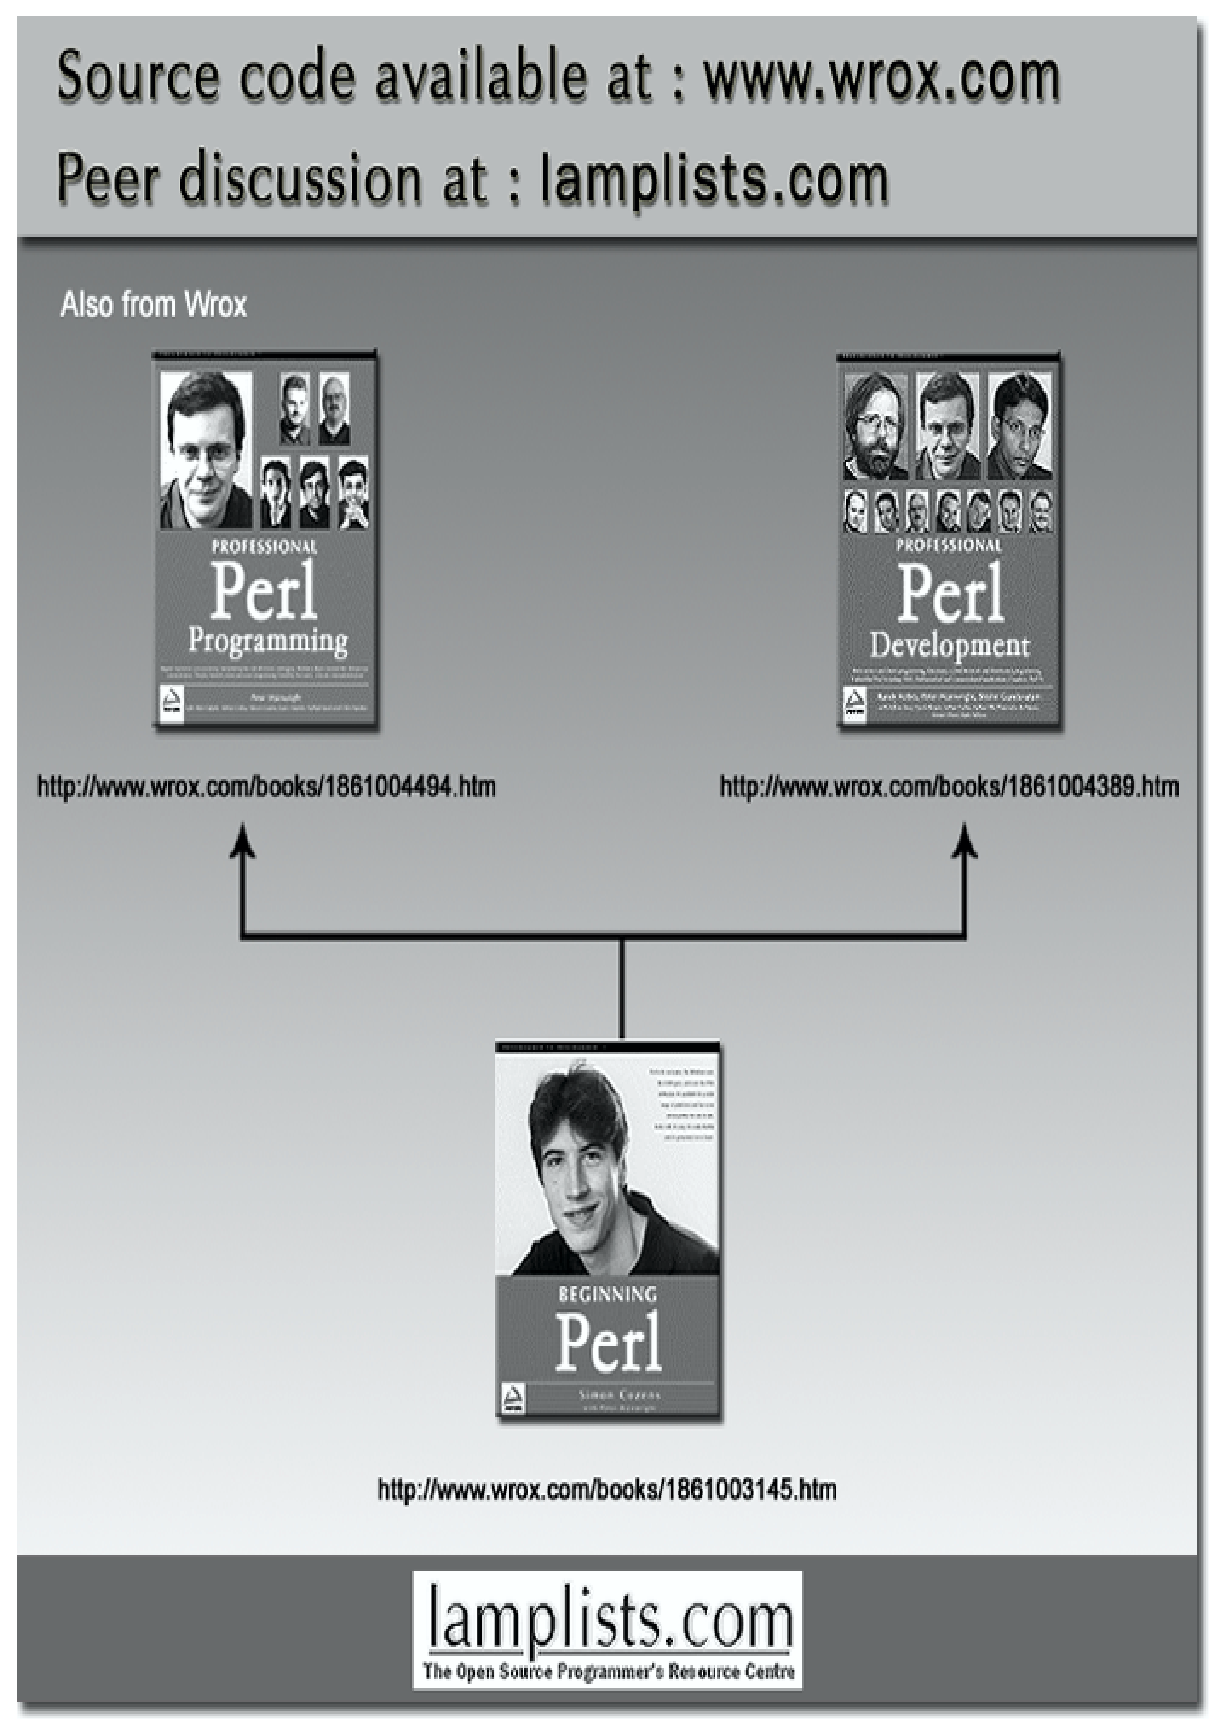
\includegraphics[bb=0mm 0mm 208mm 296mm, width=22.3mm, height=23.1mm, viewport=3mm 4mm 205mm 292mm]{image4.ps}Function Reference

\noindent 

\noindent 

\noindent 

\noindent 

\noindent Below you'll find an alphabetical list of every function in Perl 5.6 starting with a runthrough of the file

\noindent tests which are themselves functions. Marked against each function will be the syntax for the function, a brief description of what it does and any directly related functions.

\noindent 

\noindent File Tests

\noindent 

\noindent \textbf{Function Syntax Description}

\noindent 

\noindent -X (file tests) -X \textit{filehandle}

\noindent 

\noindent -X \textit{expression}

\noindent 

\noindent -X

\noindent 

\noindent Runs a file test, as described in Chapter 6, determined by X, where X is one of the following letters: ABCMORSTWX bcdefgkloprstuwxz

\noindent 

\noindent If the filehandle or expression arument is omitted, the file test checks against \$\_, with the exception of -t, which

\noindent tests STDIN.

\noindent 

\noindent 

\noindent Here's a complete rundown of what each file test checks for.

\noindent 

\noindent 

\noindent \textbf{Test Meaning}

\noindent 

\noindent -A How long in days between the last access to the file and latest startup.

\noindent 

\noindent -B True if the file is a binary file, (compare with -T).

\noindent 

\noindent -C How long in days between the last inode change and latest startup.

\noindent 

\noindent -M How long in days between the last modification to the file and latest startup.

\noindent 

\noindent -O True if the file is owned by a real uid/gid.

\noindent 

\noindent -R True if the file is readable by a real uid/gid.

\noindent 

\noindent -S True if the file is a socket.

\noindent 

\noindent \textit{Table continued on following page}

\noindent  

     

\noindent  

\noindent  

\noindent 

\noindent 

\begin{tabular}{|p{0.2in}|p{0.4in}|p{3.5in}|} \hline 
 & \textbf{Test} & \textbf{Meaning} \\ \hline 
 & -T & True if the file is a text file, (Compare with -B). \\ \hline 
 & -W & True if the file is writable by a real uid/gid. \\ \hline 
 & -X & True if the file is executable by a real uid/gid. \\ \hline 
 & -b & True if the file is a block special file. \\ \hline 
 & -c & True if the file is a character special file. \\ \hline 
 & -d & True if the file is a directory. \\ \hline 
 & -e & True if the file exists. \\ \hline 
 & -f & True if the file is a plain file - not a directory. \\ \hline 
 & -g & True if the file has the setgid bit set. \\ \hline 
 & -k & True if the file has the sticky bit set. \\ \hline 
 & -l & True if the file is a symbolic link. \\ \hline 
 & -o & True if the file is owned by an effective uid/gid. \\ \hline 
 & -p & True if the file is a named pipe or if the filehandle is a named pipe. \\ \hline 
 & -r & True if the file is readable by an effective uid/gid. \\ \hline 
 & -s & True if the file has nonzero size - returns size of file in bytes. \\ \hline 
 & -t & True if the filehandle is opened to a tty. \\ \hline 
 & -u & True if the file has the setuid bit set. \\ \hline 
 & -w & True if the file is writable by an effective uid/gid. \\ \hline 
 & -x & True if the file is executable by an effective uid/gid. \\ \hline 
 & -z & True if the file has zero size. \\ \hline 
\newline \textit{A} &  &  \\ \hline 
\end{tabular}



\noindent \textbf{Function Syntax Description}

\noindent 

\noindent abs abs \textit{value}

\noindent 

\noindent abs

\noindent 

\noindent 

\noindent 

\noindent 

\noindent accept accept \textit{newsocket, genericsocket}

\noindent 

\noindent Returns the absolute (non-negative) value of an integer. E.g. abs(-1) and abs both return 1 as a reuslt.

\noindent 

\noindent If no \textit{value }argument is given, abs returns the absolute value of \$\_.

\noindent 

\noindent Accepts an incoming socket connect with sessions enabled, if applicable.

\noindent 

\noindent alarm alarm \textit{num\_seconds}

\noindent alarm

\noindent 

\noindent Starts a timer with \textit{num\_seconds }seconds on the clock before it trips a SIGALRM signal. Before the timer runs out, another call to alarm cancels it and starts a new timer with num\_seconds on the clock. If num\_seconds equals zero, the previous timer is cancelled without starting a new one.

\noindent atan2 atan2 \textit{x, y }Returns the arctangent of \textit{x}/\textit{y }within the range - to .

\noindent 

\noindent 

\noindent \textit{B}

\noindent 

\noindent \textbf{Function Syntax Description}

\noindent 

\noindent bind bind \textit{socket}, \textit{name }Binds a network address (TCP/IP, UDP, etc) to a \textit{socket}, where \textit{name }should be the packed address for the socket.

\noindent 

\noindent binmode binmode \textit{filehandle }Sets the specified \textit{filehandle }to be read in binary mode explicitly for those systems that cannot do this automatically. Unix and MacOS can, and thus binmode has no effect under these OS's.

\noindent bless bless \textit{ref, classname}

\noindent 

\noindent bless \textit{ref}

\noindent 

\noindent Takes the variable referenced by \textit{ref }and makes it an object of class \textit{classname}.

\noindent 

\noindent 

\noindent \textit{C}

\noindent 

\noindent \textbf{Function Syntax Description}

\noindent 

\noindent caller caller \textit{expression}

\noindent caller

\noindent 

\noindent 

\noindent 

\noindent 

\noindent chdir chdir \textit{new\_directory}

\noindent chdir

\noindent 

\noindent Called within a subroutine, caller returns a list of information outlining what called it - the sub's context. Actually returns the caller's package name, its filename and line number of the call. Returns the undefined value

\noindent if not in a subroutine. If \textit{expression }is used, also returns some extra debugging information to make a stack trace.

\noindent Changes your current working directory to \textit{new\_directory}. If \textit{new\_directory }is omitted, the working directory is changed to that one specified in \$ENV(HOME).

\noindent chmod chmod \textit{list }Changes the permissions on a list of files. The first element of \textit{list }must be the octal representation of the permissions to be given those files.

\noindent chomp chomp \textit{variable }chomp \textit{list }chomp

\noindent 

\noindent Usually removes \textbackslash n from a string. Actually removes the trailing record separator as set in \$/ from a string or

\noindent from each string in a list, and then returns the number of characters deleted. If no argument is given, chomp acts

\noindent on \$\_.

\noindent 

\noindent 

\noindent \textbf{Function Syntax Description}

\noindent 

\noindent chop chop \textit{variable}

\noindent 

\noindent chop \textit{list}

\noindent 

\noindent chop

\noindent 

\noindent Removes the last character from a string or from each string in a list, and returns the (last) character chopped. If no argument is given, chop acts on \$\_.

\noindent 

\noindent chown chown \textit{list }Changes the ownership on a list of files. Within \textit{list}, the first two elements must be the user id and group

\noindent id of that user and group to get ownership, followed by any number of filenames. Setting -1 for either id means, 'Leave this value unchanged.'

\noindent 

\noindent chr chr \textit{number}

\noindent 

\noindent chr

\noindent 

\noindent chroot chroot \textit{directory}

\noindent 

\noindent chroot

\noindent 

\noindent close close \textit{filehandle}

\noindent 

\noindent close

\noindent 

\noindent Returns ASCII character number \textit{number }as determined by Appendix F. If \textit{number }is omitted, \$\_ is used.

\noindent 

\noindent Changes the root directory for all further path lookups to \textit{directory}. If \textit{directory }is not given, \$\_ is used as the new root directory.

\noindent 

\noindent Closes the file, pipe, or socket associated with the nominated \textit{filehandle}, resetting the line counter \$. as well. If \textit{filehandle }is not given, closes the currently selected filehandle. Returns true on success.

\noindent 

\noindent closedir closedir \textit{dirhandle }Closes the directory opened by opendir()   given by

\noindent \textit{dirhandle}.

\noindent 

\noindent connect connect \textit{socket, address}

\noindent 

\noindent Tries to connect to a \textit{socket }at the given \textit{address}.

\noindent 

\noindent cos cos \textit{num\_in\_radians }Calculates and returns the cosine of a number given

\noindent in radians. If \textit{num\_in\_radians }is not given, calculates the cosine of \$\_.

\noindent 

\noindent crypt crypt \textit{plaintext, key }A one-way encryption function (there is no decrypt function) that takes some \textit{plaintext }(a password usually) and encrypts it with a two character \textit{key}.

\noindent 

\noindent 

\noindent \textit{D}

\noindent 

\noindent \textbf{Function Syntax Description}

\noindent 

\noindent dbmclose dbmclose \textit{hash }Deprecated in favor of untie().

\noindent 

\noindent Breaks the binding between a dbm file and the given

\noindent \textit{hash}.

\noindent 

\noindent dbmopen dbmopen \textit{hash, dbname, mode}

\noindent 

\noindent 

\noindent 

\noindent 

\noindent 

\noindent defined defined \textit{expression}

\noindent 

\noindent defined

\noindent 

\noindent delete delete \textit{\$hash}\{\textit{key\}}

\noindent 

\noindent delete @hash\textit{\{keys}

\noindent \textit{\%hash\}}

\noindent 

\noindent Deprecated in favor of tie().

\noindent 

\noindent Binds the specified \textit{hash }to the database \textit{dbname}. If the database does not exist, it is created with the specified read\textbackslash write \textit{mode}, given as an octal number.

\noindent 

\noindent Checks whether the value, variable, or function

\noindent in \textit{expression }is defined. If \textit{expression }is omitted, \$\_

\noindent is checked.

\noindent 

\noindent Deletes one or more specified \textit{key }and corresponding value from the \textit{hash. }Returns the associated value(s).

\noindent 

\noindent die die \textit{message }Writes \textit{message }to the standard error output and

\noindent then exits the currently running program with \$!

\noindent as its return value.

\noindent 

\noindent do do \textit{filename }Executes the contents of \textit{filename }as a perl script.

\noindent Returns undef if it cannot read the file.

\noindent 

\noindent Note: do \textit{block }is not a function.

\noindent 

\noindent dump dump \textit{label}

\noindent 

\noindent dump

\noindent 

\noindent Initiates a core dump to be undumped into a new binary executable file, which when run will start at \textit{label}. If \textit{label }is left out, the executable will start

\noindent from the top of the file.

\noindent 

\noindent 

\noindent \textit{E}

\begin{tabular}{|p{1.1in}|p{0.9in}|p{2.2in}|} \hline 
\textbf{Function} & \textbf{Syntax} & \textbf{Description} \\ \hline 
each & each \textit{hash} & Returns the next key/value pair from a \textit{hash }as a \\ \hline 
 &  & two-element list. When \textit{hash }is fully read, returns \\ \hline 
 &  & null. \\ \hline 
endgrent & engrent & Frees the resources used to scan the \\ \hline 
 &  & /etc/group file or system equivalent. \\ \hline 
endhostent & endhostent & Frees the resources used to scan the \\ \hline 
 &  & /etc/hosts file or system equivalent. \\ \hline 
endnetent & endnetent & Frees the resources used to scan the \\ \hline 
 &  & /etc/networks file or system equivalent. \\ \hline 
endprotoent & endprotoent & Frees the resources used to scan the \\ \hline 
 &  & /etc/protocols file or system equivalent. \\ \hline 
\end{tabular}



\noindent 

\noindent \textbf{Function Syntax Description}

\noindent 

\noindent endpwent endpwent Frees the resources used to scan the /etc/passwd

\noindent file or system equivalent.

\noindent 

\noindent endservent endservent Frees the resources used to scan the

\noindent /etc/services file or system equivalent.

\noindent 

\noindent eof eof \textit{filehandle}

\noindent eof()

\noindent eof

\noindent 

\noindent 

\noindent 

\noindent eval eval \textit{string }eval \textit{block }eval

\noindent 

\noindent Returns 1 if \textit{filehandle }is either not open or will return end of file on next read. eof() checks for

\noindent the end of the pseudo file containing the files listed

\noindent on the command line as program was run. If eof does not have an argument, it will check the lst file to be read.

\noindent 

\noindent Parses and executes \textit{string }as if it were a mini- program and returns its result. If no argument is given, it evaluates \$\_. If an error occurs or die() is called eval, returns undef. Works similarly with \textit{block }except eval \textit{block }is parsed only once. eval \textit{string }is reparsed each time eval executes.

\noindent exec exec \textit{command }Abandons the current program to run the specified system \textit{command}.

\noindent 

\noindent exists exists \textit{\$hash\{\$key\} }Returns true if the specified \textit{key }exists within the specified \textit{hash}.

\noindent exit exit \textit{status }Terminates current program immediately with return value \textit{status}. (N.B. The only universally

\noindent recognized return values are 1 for failure and 0 for success.)

\noindent exp exp \textit{number }Returns the value of e to the power of \textit{number }(or \$\_

\noindent if number is omitted).

\noindent 

\noindent \textit{F}

\noindent 

\noindent \textbf{Function Syntax Description}

\noindent 

\noindent fcntl fcntl  \textit{filehandle, function, args}

\noindent 

\noindent Calls the fcntl function, to use on the file or device opened with \textit{filehandle}.

\noindent fileno fileno \textit{filehandle }Returns the file descriptor for \textit{filehandle.}

\noindent flock flock \textit{filehandle, locktype }Tries to lock or unlock a write-enabled file for use

\noindent by the program. Note that this lock is only advisory and that other systems not supporting flock will be able to write to the file. \textit{locktype }can take one of four values; LOCK\_SH (new shared lock), LOCK\_EX (new exclusive lock), LOCK\_UN (unlock file), and

\noindent LOCK\_NB (do not block access to the file for a new

\noindent lock if file not instantly available). Returns true for success, false for failure.

\noindent  

\noindent  

\noindent 

\noindent fork fork System call that creates a new system

\noindent process also running this program from the same point the fork was called. Returns the new process' id to the original program, 0 to the new process, or undef if the fork did

\noindent not succeed.

\noindent 

\noindent format format Declares an output template for use with

\noindent write().

\noindent 

\noindent formline formline \textit{template, list }An internal function used for formats.

\noindent Applies \textit{template }to the \textit{list }of values and stores the result in \$\^{}A. Always returns true.

\noindent 

\noindent 

\noindent \textit{G}

\noindent 

\noindent \textbf{Description}

\noindent 

\noindent Waits for the user to press Return and then retrieves the next character from \textit{filehandle}'s file. Returns undef if at the end of a file. If \textit{filehandle }is omitted, uses STDIN instead.

\noindent 

\noindent Gets the next group record from

\noindent /etc/group or the system equivalent, returning an empty record when the end of the file is reached.

\noindent 

\noindent Gets the group record from /etc/group or the system equivalent whose id field matches the given group number \textit{gid. }Returns an

\noindent empty record if no match occurs.

\noindent 

\noindent Gets the group record from /etc/group or the system equivalent whose name field matches the given group \textit{name. }Returns an empty record if no match occurs.

\noindent 

\noindent Returns the hostname for a packed binary network \textit{address }of a certain address type. By default, \textit{addrtype }is assumed to be IP.

\noindent 

\noindent Returns the network address given its

\noindent corresponding \textit{hostname}.

\noindent 

\noindent \textit{Table continued on following page}

\noindent 

\noindent 

\noindent \textbf{Description}

\noindent 

\noindent Gets the next network host record from

\noindent /etc/hosts or the system equivalent, returning an empty record when the end of the file is reached.

\noindent 

\noindent Returns the user id for the currently logged in user.

\noindent 

\noindent Returns the net name for a given network \textit{address }of a certain address type. By default, \textit{addrtype }is assumed to be IP.

\noindent 

\noindent Returns the net address given its corresponding net \textit{name}.

\noindent 

\noindent Gets the next entry from

\noindent /etc/networks or the system equivalent, returning an empty record when the end of the file is reached.

\noindent getpeername getpeername \textit{socket }Returns the address for the other end of the connection to this \textit{socket}.

\noindent getpgrp getpgrp \textit{process\_id}

\noindent getpgrp

\noindent 

\noindent Returns the process group in which the specified process is running. Assumes current process if \textit{process\_id }is not given.

\noindent getppid getppid Returns the process id of the current process' parent process.

\noindent getpriority getpriority \textit{type, id }Returns current priority for a process, process group, or user as determined by \textit{type}.

\noindent getprotobyname getprotobyname \textit{name }Returns the number for the protocol given in \textit{name}.

\noindent getprotobynumber getprotobynumber

\noindent \textit{number}

\noindent 

\noindent Returns the name of the protocol given its \textit{number}.

\noindent getprotoent getprotoent Gets the next entry from

\noindent /etc/protocols or the system equivalent, returning an empty record when the end of the file is reached.

\noindent getpwent getpwent Gets the next entry from /etc/passwd

\noindent or the system equivalent, returning an empty record when the end of the file is reached.

\noindent getpwnam getpwnam \textit{name }Gets the password record whose login name field matches the given \textit{name. }Returns an empty record if no match occurs.

\noindent 

\noindent getpwuid getpwuid \textit{uid }Gets the password record whose user id field matches the given \textit{uid. }Returns an empty record if no match occurs.

\noindent getservbyname getservbyname \textit{name, protocol}

\noindent 

\noindent getservbyport getservbyport \textit{port, protocol}

\noindent 

\noindent Returns the port number for the \textit{name}d service on the given \textit{protocol}.

\noindent 

\noindent Returns the port name for the service \textit{port}

\noindent on the given \textit{protocol}.

\noindent 

\noindent getservent getservent Gets the next entry from

\noindent /etc/services or the system equivalent, returning an empty record when the end of the file is reached.

\noindent getsockname getsockname \textit{socket }Returns the address for this end of the connection to this \textit{socket}.

\noindent getsockopt getsockopt \textit{socket, level,optname}

\noindent glob glob \textit{expression}

\noindent glob

\noindent 

\noindent Returns the specified socket option or

\noindent undef if an error occurs.

\noindent 

\noindent Returns a list of filenames matching the regular \textit{expression }in the current directory. If \textit{expression }is omitted, the comparison is made with \$\_.

\noindent gmtime gmtime Returns a nine-element integer array representing the given \textit{time }(or time() if not given) converted to GMT. By index order, the nine elements (all zero-based) represent:

\noindent 0 Number of seconds in the current minute.

\noindent 

\noindent 

\noindent 1 Number of minutes in the current hour.

\noindent 

\noindent 

\noindent 2 Current hour.

\noindent 

\noindent 

\noindent 3 Current day of month.

\noindent 

\noindent 

\noindent 4 Current month.

\noindent \textit{Table continued on following page}

\noindent 

\noindent 

\noindent \textbf{Function Syntax Description}

\noindent 

\noindent gmtime (cont.) gmtime \textit{time }(cont.) 5 Number of years since 1900

\noindent 

\noindent 

\noindent 6 Weekday (Sunday = 0)

\noindent 

\noindent 

\noindent 7 Number of days since January 1.

\noindent 

\noindent 

\noindent 

\noindent 

\noindent 

\noindent goto goto \textit{tag}

\noindent 

\noindent goto \textit{expression}

\noindent 

\noindent goto \textit{\&subroutine}

\noindent 

\noindent 

\noindent 

\noindent 

\noindent 

\noindent 

\noindent 

\noindent grep grep \textit{expression, list}

\noindent 

\noindent grep \textit{\{block\} list}

\noindent 8  Whether daylight savings time is in

\noindent effect.

\noindent 

\noindent Looks for \textit{tag }either given literally or dynamically derived by resolving expression and resumes execution of the program there on the provision that it is not inside a construct that requires initializing. For example, a for loop.

\noindent Alternatively, goto \textit{\&subroutine }switches a call to \textit{subroutine }for the currently running subroutine.

\noindent 

\noindent Evaluates a given \textit{expression }or \textit{block }of code against each element in \textit{list }and returns a list of those elements for which the evaluation returned true.

\noindent 

\noindent \textit{H}

\noindent 

\noindent \textbf{Function Syntax Description}

\noindent 

\noindent hex hex \textit{string}

\noindent 

\noindent hex

\noindent 

\noindent Reads in \textit{string }as a hexadecimal number and returns the corresponding decimal equivalent. Uses \$\_ if string is omitted.

\noindent 

\noindent 

\noindent \textit{I}

\noindent 

\noindent \textbf{Function Syntax Description}

\noindent 

\noindent import import \textit{module list}

\noindent 

\noindent import \textit{module}

\noindent 

\noindent Patches a module's namespace into your own, incorporating the \textit{list}ed

\noindent subroutines and variables into your own package (or all of them if \textit{list }isn't given).

\noindent 

\noindent 

\noindent index index \textit{string, substring, position}

\noindent 

\noindent index \textit{string, substring}

\noindent 

\noindent int int \textit{number}

\noindent 

\noindent int

\noindent 

\noindent ioctl ioctl \textit{filehandle, function, argument}

\noindent 

\noindent Returns the zero-based position of \textit{substring }in \textit{string}

\noindent first occuring after character number \textit{position}.

\noindent Assumes \textit{position }equals zero if not given. Returns -1

\noindent if match not found.

\noindent 

\noindent Returns the integer section of \textit{number }or \$\_ if \textit{number}

\noindent is omitted.

\noindent 

\noindent Calls the ioctl function, to use on the file or device opened with \textit{filehandle}.

\noindent 

\noindent 

\noindent \textit{J}

\noindent 

\noindent \textbf{Function Syntax Description}

\noindent 

\noindent join join \textit{character}, \textit{list }Returns a single string comprising the elements of

\noindent \textit{list}, separated from each other by \textit{character.}

\noindent 

\noindent 

\noindent \textit{K}

\noindent 

\noindent \textbf{Function Syntax Description}

\noindent 

\noindent keys keys \textit{hash }Returns a non-ordered list of the keys contained in

\noindent \textit{hash}.

\noindent 

\noindent kill kill \textit{signal}, \textit{process\_list }Sends a \textit{signal }to the processes and/or process groups

\noindent in process\_list. Returns number of signals successfully sent.

\noindent 

\noindent 

\noindent \textit{L}

\noindent 

\noindent \textbf{Function Syntax Description}

\noindent 

\noindent last last \textit{label}

\noindent 

\noindent last

\noindent 

\noindent Causes the program to break out of the \textit{label}ed loop (or the innermost loop, if \textit{label }is not given) surrounding the command and to continue with the statement immediately following the loop.

\noindent 

\noindent lc lc \textit{string }Returns \textit{string }in lower case or \$\_ in lower case if

\noindent \textit{string }is omitted.

\noindent 

\noindent lcfirst lcfirst \textit{string }Returns \textit{string }with the first character in lower case.

\noindent Works on \$\_ if \textit{string }is omitted.

\noindent \textit{Table continued on following page}

\noindent 

\noindent 

\noindent \textbf{Function Syntax Description}

\noindent 

\noindent length length \textit{expression }Evaluates \textit{expression }and returns the number of characters in that value. Returns length \$\_ if

\noindent \textit{expression }is omitted.

\noindent 

\noindent link link \textit{thisfile}, \textit{thatfile }Creates a hard link in the filesystem, from \textit{thatfile }to

\noindent \textit{thisfile}. Returns true on sucess, false on failure.

\noindent 

\noindent listen listen \textit{socket},

\noindent \textit{max\_connectons}

\noindent 

\noindent Listens for connections to a particular \textit{socket }on a server and reports when the number of connections exceeds \textit{max\_connections}.

\noindent local local \textit{var }Declares a 'private' variable that is available to the subroutine in which it is declared and any other subroutines that may be called by this subroutine.

\noindent 

\noindent Actually creates a temporary value for a global variable for the duration of the subroutine's execution.

\noindent localtime localtime \textit{time }Returns a nine-element array representing the given

\noindent \textit{time }(or time() if not given) converted to system local time. See gmtime() for desription of elements.

\noindent log log \textit{number }Returns the natural logarithm for a \textit{number}. That is, returns \textit{x }where e\textit{x}=\textit{number.}

\noindent 

\noindent lstat lstat \textit{filehandle}

\noindent 

\noindent lstat \textit{expression}

\noindent lstat

\noindent 

\noindent Returns a thirteen element status array for the symbolic link to a file and not the file itself. See stat() for further details.

\noindent 

\noindent \textit{M}

\noindent 

\noindent \textbf{Function Syntax Description}

\noindent 

\noindent m// m// Tries to match a regular expression pattern against a string.

\noindent map map \textit{expression, list}

\noindent 

\noindent map \textit{\{block\} list}

\noindent 

\noindent Evaluates a given \textit{expression }or \textit{block }of code against each element in \textit{list }and returns a list of the results of each evaluation.

\noindent mkdir mkdir \textit{dirname, mode }Creates a directory called \textit{dirname }and gives it the read\textbackslash write permissions as specified in \textit{mode }(an octal number).

\noindent msgctl msgctl \textit{id, cmd, arg }Calls the System V IPC msgctl function.

\noindent msgget msgget \textit{key, flags }Calls the System V IPC msgget function.

\noindent 

\noindent msgrcv msgrcv \textit{id, var, size, type, flags}

\noindent 

\noindent Calls the System V IPC msgrcv function.

\noindent 

     

\noindent  

\noindent 

\noindent 

\noindent \textbf{Description}

\noindent 

\noindent Calls the System V IPC msgsnd function.

\noindent 

\noindent Declares the variables in \textit{variable\_list }to be lexically local to the block or file it has been declared in.

\noindent 

\noindent 

\noindent 

\noindent 

\noindent \textbf{Description}

\noindent 

\noindent Causes the program to start the next iteration of the \textit{label}led loop (or the innermost loop, if \textit{label }is not given) surrounding the command.

\noindent Removes the functionality and semantics of the named module from the current package. Compare with use() which does the opposite.

\noindent 

\noindent 

\noindent 

\noindent 

\noindent \textbf{Description}

\noindent 

\noindent Reads in \textit{string }as an octal number and returns the corresponding decimal equivalent. Uses \$\_ if

\noindent string is omitted.

\noindent 

\noindent Opens the file called \textit{filename }and associates it with \textit{filehandle}. If \textit{filename }is omitted, open assumes that the file has the same name as \textit{filehandle}.

\noindent 

\noindent Opens the directory called \textit{dirname }and associates it with \textit{dirhandle}.

\noindent 

\noindent Returns the numerical ASCII value of the first character in \textit{expression}.

\noindent 

\noindent 

\noindent 

\noindent 

\noindent \textbf{Description}

\noindent 

\noindent Takes a \textit{list }of values and puts them into a binary structure using \textit{template }(a sequence of characers as shown below) to give the structure an ordered composition. The possible characters for \textit{template}

\noindent are:

\noindent 

\noindent 

\noindent \textit{Table continued on following page}

\noindent 

\noindent pack (cont.) pack \textit{template, list }(cont.) a Null-padded ASCII string A Space-padded ASCII

\noindent string.

\noindent 

\noindent b A bit string (low-to-high). B A bit string (high-to-low). c A signed char value.

\noindent C An unsigned char value.

\noindent 

\noindent d A double-precision float in the native format.

\noindent 

\noindent f A single-precision float in the native format. h A hexadecimal string, low to high.

\noindent H A hexadecimal string, high to low.

\noindent 

\noindent i A signed integer.

\noindent 

\noindent I An unsigned integer. l A signed long value.

\noindent L An unsigned long value.

\noindent 

\noindent n A big-endian short (16-bit) value. N A big-endian long (32-bit) value.

\noindent p A pointer to a null-terminated string.

\noindent 

\noindent P A pointer to a fixed-length string. q A signed quad (64-bit) value.

\noindent Q An unsigned quad (64-bit) value. s A signed short (16-bit) value.

\noindent S An unsigned short (16-bit) value.

\noindent 

\noindent v A little-endian short (16-bit) value. V A big-endian long (32-bit) value.

\noindent u A uuencoded string.

\noindent 

\noindent w A BER compressed integer - an unsigned integer in base 128, high-bit first.

\noindent 

\noindent x A null byte.

\noindent 

\noindent X Back up a byte.

\noindent 

\noindent 

\noindent \textbf{Description}

\noindent 

\noindent Z A null-padded, null-terminated string.

\noindent 

\noindent @ Null-fill to absolute position.

\noindent 

\noindent Declares that the following block of code is to be defined within the specified \textit{namespace}.

\noindent 

\noindent Opens and connects two filehandles, such that the pipe reads content from \textit{readhandle }and passes it to \textit{writehandle}.

\noindent 

\noindent Removes and returns the last element (at largest index position) from \textit{array. }Pops @ARGV if \textit{array }is not specified.

\noindent 

\noindent Returns the position in \textit{scalar }of the character following the last m//g match. Uses \$\_ for \textit{scalar }if omitted.

\noindent 

\noindent Prints a \textit{list }of comma-separated strings to the file associated with \textit{filehandle }or STDOUT if not specified. If both arguments are omitted, prints \$\_ to the currently selected output channel.

\noindent 

\noindent As print() but prints to the output channel using

\noindent a specified \textit{format}.

\noindent 

\noindent 

\noindent Returns the prototype of a \textit{function }as a string or

\noindent undef if the prototype does not exist.

\noindent 

\noindent Adds the elements of \textit{list }to the \textit{array }at position max\_index.

\noindent 

\noindent 

\noindent 

\noindent 

\noindent \textbf{Description}

\noindent 

\noindent Alternative method of putting single quotes around

\noindent a string.

\noindent 

\noindent Alternative method of putting double quotes around a string.

\noindent 

\noindent Scans through \textit{expression }and returns it having prefixed all non-alphanumeric or  -underscore characters with a backslash.

\noindent \textit{Table continued on following page}

\noindent 

\noindent qw// qw/\textit{strings}/ Returns a list of strings, the elements of which are created by splitting a \textit{string }by whitespace

\noindent or the \textit{strings }sent to qw//.

\noindent qx// qx/\textit{string}/ Alternative method of backtick-quoting a \textit{string}

\noindent (which now acts as a command-line command.

\noindent 

\noindent 

\noindent \textit{R}

\noindent 

\noindent \textbf{Function Syntax Description}

\noindent 

\noindent rand rand \textit{expression }Evaluates expression and then returns a random value \textit{x }where 0 $<$= \textit{x }$<$ the value of

\noindent \textit{expression}.

\noindent 

\noindent read read \textit{filehandle, scalar, length, offset}

\noindent 

\noindent read \textit{filehandle, scalar, length}

\noindent 

\noindent Reads \textit{length }number of bytes in from \textit{filehandle}, placing them in \textit{scalar}. Starts by default from

\noindent the start of the file, but you can specify \textit{offset},

\noindent the position in the file you wish to start reading from. Returns the number of bytes read, zero if at the end of the file or undef if file doesn't exist.

\noindent readdir readdir \textit{dirhandle }Returns the next entry in the directory specified by \textit{dirhandle }or if being used in list context, the entire contents of the directory.

\noindent readline readline \textit{filehandle }Returns a line from \textit{filehandle}'s file if in scalar context or returns a list containing all the lines

\noindent of the file as its elements.

\noindent 

\noindent readlink readlink \textit{linkname }Returns the name of the file at the end of symbolic link \textit{linkname}.

\noindent readpipe readpipe \textit{command }Executes \textit{command }on the command line and then returns the standard output generated by

\noindent it as a string. Returns a list of lines from the standard output if in list context.

\noindent recv recv \textit{socket, scalar, length, flags}

\noindent 

\noindent redo redo \textit{label}

\noindent redo

\noindent 

\noindent 

\noindent 

\noindent ref ref \textit{reference}

\noindent ref

\noindent 

\noindent Receives a \textit{length }byte message over the named

\noindent \textit{socket }and reads it into a \textit{scalar }string.

\noindent 

\noindent Causes the program to restart the current iteration of the \textit{label}ed loop (or the innermost loop, if \textit{label }is not given) surrounding the command without checking the while condition.

\noindent 

\noindent Returns the type of object being referenced by \textit{reference }or a package name if the object has been blessed into a package.

\noindent 

\noindent 

\noindent 

\noindent \textbf{Function Syntax Description}

\noindent 

\noindent rename rename \textit{oldname, newname }Renames file \textit{oldname }as \textit{newname. }Returns 1 for success or 0 if otherwise.

\noindent require require \textit{file }require \textit{package }require \textit{num}

\noindent require

\noindent 

\noindent Ensures that the named \textit{package }or \textit{file }are included at runtime. If \textit{num }is argument, ensure that version of Perl currently running is greater than or equal to \textit{num }(or \$\_ if omitted).

\noindent reset reset \textit{expression }Resets all variables in current package beginning with one of the characters in

\noindent \textit{expression }and all ?? searches to their original state.

\noindent return return \textit{expression }Returns the value of \textit{expression }from a subroutine or eval().

\noindent reverse reverse \textit{list }Returns either \textit{list }with its elements in reverse order if in list context or a string consisting of the elements of \textit{list }concatenated together and then written backwards.

\noindent rewinddir rewinddir \textit{dirhandle }Resets the point of access for readdir()to the top of directory \textit{dirhandle}.

\noindent rindex rindex \textit{string, substring, position}

\noindent 

\noindent rindex \textit{string, substring}

\noindent 

\noindent Returns the zero-based position of the last occurence of \textit{substring }in \textit{string }at or before character number \textit{position}. Returns -1 if match not found.

\noindent rmdir rmdir \textit{dirname }If directory \textit{dirname }(or that given in \$\_ if omitted) is empty, it is removed. Returns true on success or false if otherwise.

\noindent 

\noindent \textit{S}

\noindent 

\noindent \textbf{Function Syntax Description}

\noindent 

\noindent s/// s/\textit{matchstring}/\textit{replacestring}/ Searches for \textit{matchstring }in \$\_ and replaces it with \textit{replacestring }if found.

\noindent scalar scalar \textit{expression }Evaluates \textit{expression }in scalar context and returns the resultant value.

\noindent seek seek \textit{filehandle, position, flag}

\noindent 

\noindent Sets the \textit{position }(character number) in a file denoted by \textit{filehandle }from which the file will

\noindent be read/written. \textit{Flag }tells seek whether to goto character number \textit{position }(\textit{flag }= 0), number current position + \textit{position }(\textit{flag }= 1) or number EOF + \textit{position }(\textit{flag}=2). Returns 1 on success or

\noindent 0 if otherwise.

\noindent \textit{Table continued on following page}

     

\noindent  

\noindent 

\noindent seekdir seekdir \textit{dirhandle, position }Sets the \textit{position }(entry number) in a

\noindent directory denoted by \textit{dirhandle }from which directory entries will be read.

\noindent 

\noindent select select \textit{filehandle}

\noindent 

\noindent select

\noindent 

\noindent 

\noindent select select \textit{rbits, wbits, ebits, timeout}

\noindent 

\noindent 

\noindent 

\noindent 

\noindent semctl semctl \textit{id, sem\_num, command, argument}

\noindent 

\noindent semget semget \textit{id, semnum, command, argument}

\noindent 

\noindent Changes the current default filehandle (starts as STDOUT) to \textit{filehandle}. Returns the current default filehandle if \textit{filehandle }is omitted.

\noindent 

\noindent Calls the system select command to wait for \textit{timeout }seconds until one (if any) of your filehandles become available for reading or writing and returns either success or failure.

\noindent 

\noindent Calls the System V IPC semctl function.

\noindent 

\noindent 

\noindent Calls the System V IPC semget function.

\noindent 

\noindent semop semop \textit{key, opstring }Calls the System V IPC semop function.

\noindent 

\noindent send send \textit{socket, message, flags, destination}

\noindent 

\noindent send \textit{socket, message, flags}

\noindent 

\noindent setpgrp setpgrp \textit{process\_id, process\_group}

\noindent 

\noindent 

\noindent setpriority setpriority \textit{which, id, priority}

\noindent 

\noindent 

\noindent 

\noindent setsockopt setsockopt \textit{socket, level, option, optional\_value}

\noindent 

\noindent shift shift \textit{array}

\noindent 

\noindent shift

\noindent 

\noindent 

\noindent 

\noindent 

\noindent shmctl shmctl \textit{id, command, argument}

\noindent 

\noindent Sends a \textit{message }from a \textit{socket }to the connected socket, or, if \textit{socket }is disconnected, to \textit{destination}. Takes account of any system \textit{flags }given it.

\noindent 

\noindent Sets the \textit{process\_group }in which the process with the given \textit{process\_id }should run. The arguments default to 0 if not given.

\noindent 

\noindent Adds to or diminshes the priority of either a process, process group, or user, as determined by \textit{which }and specifically identified by its \textit{id}.

\noindent 

\noindent Sets the \textit{option }for the given \textit{socket}. Returns

\noindent undef if an error occurs.

\noindent 

\noindent 

\noindent Returns the element at position 0 in array and then removes it from array. Returns undef if there are no elements in the array. Shifts @\_ within subroutines and formats or @ARGV otherwise if \textit{array }is omitted.

\noindent 

\noindent Calls the System V IPC shmctl function.

\noindent 

\noindent 

\noindent 

\begin{tabular}{|p{0.9in}|p{1.3in}|p{2.0in}|} \hline 
\textbf{Function} & \textbf{Syntax} & \textbf{Description} \\ \hline 
shmget & shmget \textit{key, size, flags} & Calls the System V IPC shmget function. \\ \hline 
\end{tabular}

shmread shmread \textit{id, variable, position, size}

\noindent 

\noindent shmwrite shmwrite \textit{id, string, position, size}

\noindent Calls the System V IPC shmread function.

\noindent 

\noindent 

\noindent Calls the System V IPC shmwrite function.

\noindent 

\noindent shutdown shutdown \textit{socket, manner }Shuts down the \textit{socket }specified in the

\noindent following \textit{manner}.

\noindent 

\noindent 0 Stop reading data.

\noindent 

\noindent 

\noindent 

\noindent 1 Stop writing data.

\noindent 

\noindent 

\noindent 

\noindent 2 Stop using this socket altogether.

\noindent 

\noindent 

\noindent 

\noindent 

\noindent sin sin \textit{expression}

\noindent 

\noindent sin

\noindent 

\noindent sleep sleep \textit{n}

\noindent 

\noindent sleep

\noindent 

\noindent socket socket \textit{filehandle, domain, type, protocol}

\noindent 

\noindent 

\noindent 

\noindent socketpair socketpair \textit{sock1, sock2, domain, type, protocol}

\noindent 

\noindent 

\noindent 

\noindent sort sort \textit{subroutine list}

\noindent 

\noindent sort \textit{block list}

\noindent 

\noindent sort \textit{list}

\noindent Evaluates \textit{expression }as a value in radians and then returns the sine of that value. Returns the sine of \$\_ if exressino is omitted.

\noindent 

\noindent Causes the running script to 'sleep' for \textit{n}

\noindent seconds or forever if \textit{n }is not given.

\noindent 

\noindent Opens a socket and associates it to the given \textit{filehandle}. This socket exists within the given \textit{domain }of communcation, is of the given \textit{type }and uses the given \textit{protocol }to communicate.

\noindent 

\noindent Creates a pair of sockets named sock1 and sock2. These sockets exist within the given \textit{domain }of communcation, are of the given \textit{type }and use the given \textit{protocol }to communicate.

\noindent 

\noindent Takes a \textit{list }of values and returns it with the elements after being sorted into an order. If \textit{subroutine }is given, this is used to sort \textit{list}. If \textit{block }is given, this is used as an anonymous subroutine to sort \textit{list}. If neither are given, \textit{list }is sorted by simple string comparisons.

\noindent \textit{Table continued on following page}

\noindent 

\noindent 

\noindent splice splice \textit{array, offset, length, list}

\noindent 

\noindent splice \textit{array, offset, length}

\noindent 

\noindent splice \textit{array, offset}

\noindent 

\noindent 

\noindent 

\noindent 

\noindent 

\noindent 

\noindent split split \textit{/pattern/, string, limit }split \textit{/pattern/, string }split \textit{/pattern/}

\noindent split

\noindent 

\noindent Takes \textit{array }elements from index \textit{offset }to (\textit{offest+length}) and replaces them with the elements of \textit{list}, if any. If \textit{length }is removed, removes all the elements of array from index \textit{offset }onwards. If negative, leaves that many elements at the end of the array. If offset is negative, splice starts from index number (maxindex-\textit{offset}). Returns the last element removed if in scalar context or undef if nothing was removed.

\noindent 

\noindent Takes the given \textit{string }and returns it as an array of smaller strings where any instances

\noindent in the string matching \textit{pattern }have been used

\noindent as the delimiter for the array elements. If given, \textit{limit }denotes the number of times pattern will be searched for in string.

\noindent 

\noindent If \textit{string }is omitted, \$\_ is split. If \textit{pattern }is omitted, \$\_ is split by whitespace.

\noindent 

\noindent 

\noindent sprintf sprintf \textit{format, list }As printf() but prints \textit{list }to a string using

\noindent a specified \textit{format}.

\noindent 

\noindent 

\noindent 

\noindent sqrt sqrt \textit{expression}

\noindent 

\noindent sqrt

\noindent Evaluates \textit{expression }and then returns the square root of either it or \$\_ if it was left out of the call.

\noindent 

\noindent 

\noindent 

\noindent srand srand \textit{expression}

\noindent 

\noindent srand

\noindent 

\noindent stat stat \textit{filehandle }stat \textit{expression }stat

\noindent Seeds the random-number generator.

\noindent 

\noindent 

\noindent Returns a thirteen-element array comprising the following information about a file named by \textit{expression}, represented by \textit{filehandle }or contained in \$\_ (by index number).

\noindent 

\noindent 0 \$dev Device number of filesystem

\noindent 

\noindent 

\noindent 

\noindent 1 \$ino Inode number

\noindent 

\noindent 

\noindent 

\noindent \textbf{Function Syntax Description}

\noindent 

\noindent stat (cont.) stat \textit{filehandle }stat \textit{expression }stat

\noindent (cont.)

\noindent 

\noindent 

\noindent 

\noindent 

\noindent 

\noindent 

\noindent 

\noindent 

\noindent 

\noindent 

\noindent 

\noindent 

\noindent 

\noindent 

\noindent 

\noindent 

\noindent 

\noindent 

\noindent 

\noindent 

\noindent 

\noindent 

\noindent 

\noindent 

\noindent 

\noindent 

\noindent 

\noindent 

\noindent 

\noindent 

\noindent 

\noindent study study \textit{string}

\noindent 

\noindent study

\noindent 

\noindent sub sub \textit{subname block}

\noindent 

\noindent sub \textit{subname}

\noindent 

\noindent sub \textit{block}

\noindent 

\noindent 2 \$mode File mode.

\noindent 

\noindent 

\noindent 

\noindent 3 \$nlink number of links to the file.

\noindent 

\noindent 

\noindent 

\noindent 4 \$uid User id of file's owner.

\noindent 

\noindent 

\noindent 

\noindent 5 \$gid Group id of file's owner.

\noindent 

\noindent 

\noindent 

\noindent 6 \$rdev Device identifier.

\noindent 

\noindent 

\noindent 

\noindent 7 \$size Total size of file.

\noindent 

\noindent 

\noindent 

\noindent 8 \$atime Last time file was accessed.

\noindent 

\noindent 

\noindent 

\noindent 9 \$mtime Last time file was modified.

\noindent 

\noindent 

\noindent 

\noindent 10 \$ctime Last time inode was changed.

\noindent 

\noindent 

\noindent 

\noindent 11 \$blksize Preferred block size for file I/O.

\noindent 

\noindent 

\noindent 

\noindent 12 \$blocks Number of blocks allocated to file.

\noindent 

\noindent Tells perl to optimize itself for repeated searches on \textit{string }or on \$\_ if \textit{string }is omitted.

\noindent 

\noindent Declares a \textit{block }of code to be a subroutine with the name \textit{subname}. If \textit{block }is omitted, this is just a forward reference to a later declaration. If

\noindent \textit{subname }is omitted, this is an anonymous function declaration.

\noindent \textit{Table continued on following page}

\noindent  

\noindent  

\noindent 

\noindent 

\noindent 

\noindent \textbf{Function Syntax Description}

\noindent 

\noindent substr substr \textit{string, position, length, replacement}

\noindent 

\noindent substr \textit{string, position, length}

\noindent 

\noindent substr \textit{string, position}

\noindent 

\noindent Returns a substring of \textit{string }that is \textit{length }characters long, starting with the character at index number \textit{position}. If given, that substring is then silently replaced with \textit{replacement}. If

\noindent \textit{length }is not given, substr assumes the entire string from \textit{position }onwards.

\noindent 

\noindent symlink symlink \textit{oldfile, newfile }Creates \textit{newfile }as a symbolic link to \textit{oldfile}.

\noindent Returns 1 on sucess, 0 on failure.

\noindent 

\noindent syscall syscall \textit{list }Assumes the first element in the \textit{list }is the name

\noindent of a system call and calls it, taking the other elements of the \textit{list }to be arguments to that call.

\noindent 

\noindent sysopen sysopen \textit{filehandle, filename, mode, permissions}

\noindent 

\noindent sysopen \textit{filehandle, filename, mode}

\noindent 

\noindent sysread sysread \textit{filehandle, scalar, length, offset}

\noindent 

\noindent sysread \textit{filehandle, scalar, length}

\noindent 

\noindent 

\noindent 

\noindent sysseek sysseek \textit{filehandle, pos, flag}

\noindent 

\noindent Opens file \textit{filename }under the specified \textit{mode }and associates it with the given \textit{filehandle}. \textit{Permissions }is the octal value representing the permissions that you want to assign to the file. If not given, the default is 0666.

\noindent 

\noindent Reads \textit{length }number of bytes in from \textit{filehandle}, placing them in \textit{scalar }using the system call read. Starts by default from the start of the

\noindent file, but you can specify \textit{offset}, the position in

\noindent the file you wish to start reading from. Returns the number of bytes read, 0 if at the end of the file or undef if file doesn't exist.

\noindent 

\noindent Sets the system position for the file denoted by \textit{filehandle}. \textit{Flag }tells sysseek whether to goto position number \textit{pos }(\textit{flag }= 0), number current position + \textit{pos }(\textit{flag }= 1), or number EOF + \textit{pos }(\textit{flag }= 2). Returns 1 on success, 0 otherwise.

\noindent 

\noindent system system \textit{list }Forks the process that the current program is running on, lets it complete, and then

\noindent abandons the current program to run the specified system command in \textit{list}. This will be the first element of \textit{list}, and any arguments to it are stored in subsequent list elements.

\noindent 

\noindent syswrite syswrite \textit{filehandle, scalar, length, offset}

\noindent 

\noindent syswrite \textit{filehandle, scalar, length}

\noindent 

\noindent syswrite \textit{filehandle, scalar}

\noindent 

\noindent Writes \textit{length }number of bytes from the \textit{scalar }to the file denoted by \textit{filehandle}, starting at character number \textit{offset }if specified. If \textit{length }is not given, writes the entire scalar to the file.

\noindent 

\noindent 

\noindent 

\noindent \textit{T}

\noindent 

\noindent \textbf{Function Syntax Description}

\noindent 

\noindent tell tell \textit{filehandle}

\noindent 

\noindent tell

\noindent 

\noindent Returns the current read/write position for the file marked by \textit{filehandle}. If filehadle is not

\noindent given, the info is given for the last accessed file.

\noindent 

\noindent telldir telldir \textit{dirhandle }Returns the current readdir position for the directory marked by \textit{dirhandle}.

\noindent 

\noindent tie tie \textit{variable, classname, list }Binds the named \textit{variable }to package class \textit{classname}, which works on a variable of that type. Passes any arguments (in \textit{list}) to the new function of the class (TIESCALAR, TIEHASH,

\noindent or TIEARRAY).

\noindent 

\noindent tied tied \textit{variable }Returns a reference to the object tied to the given \textit{variable}.

\noindent 

\noindent time time Returns the number of non-leap seconds elpased since Jan 1, 1970. Can be translated

\noindent into recognizable time values with gmtime()

\noindent and localtime().

\noindent 

\noindent times times Returns a four-element list holding the user

\noindent and system CPU times (in seconds) for both the current process and its child processes. The list

\noindent is comprised as follows:

\noindent 

\noindent \$user

\noindent 

\noindent Current process user time.

\noindent 

\noindent \$system

\noindent 

\noindent Current process system CPU time.

\noindent 

\noindent \$cuser

\noindent 

\noindent Child process user time.

\noindent 

\noindent \$csystem

\noindent 

\noindent Child process system time.

\noindent 

\noindent tr/// tr/\textit{string1}/\textit{string2}/ Transliterates a string (also known as y///).

\noindent 

\noindent truncate truncate \textit{filehandle, length}

\noindent 

\noindent truncate \textit{expression, length}

\noindent 

\noindent Truncates the file given by \textit{filehandle }or named literally by \textit{expression }to \textit{length }characters. Returns true on success, false if otherwise.

\noindent 

\noindent 

\noindent 

\noindent \textit{U}

\noindent 

\noindent \textbf{Function Syntax Description}

\noindent 

\noindent uc uc \textit{string}

\noindent 

\noindent uc

\noindent 

\noindent Returns \textit{string }in upper case or \$\_ in upper case if \textit{string }is omitted.

\noindent 

\noindent 

\noindent ucfirst ucfirst \textit{string}

\noindent 

\noindent ucfirst

\noindent Returns \textit{string }with the first character in upper case. Works on \$\_ if \textit{string }is omitted.

\noindent 

\noindent 

\noindent umask umask \textit{expression}

\noindent 

\noindent umask

\noindent Returns the current umask and then sets it to

\noindent \textit{expression }if this is given. The umask is a

\noindent group of three octal numbers representing the access permissions for a file or directory of its owner, a group and other users, where

\noindent execute = 1, write = 2, and read = 4. So an umask of 0777 would give all permissions to all three levels of user. 0744 would restrict all except the owner to read access only.

\noindent 

\noindent 

\noindent undef undef \textit{expression}

\noindent 

\noindent undef

\noindent Removes the value of \textit{expression}, leaving it undefined, or else it just returns the undefined value.

\noindent 

\noindent unlink unlink \textit{list }Deletes the files specified in \textit{list }(or \$\_ if not given), returning the number of files deleted. (N.B. For Unix users, unlink() removes a link to each file but not the fields themselves

\noindent if other links to them still exist.)

\noindent 

\noindent 

\noindent unpack unpack \textit{template, string }The reverse of pack(). Takes a packed

\noindent \textit{string }and then uses \textit{template }to read through it and return an array of the values stored

\noindent within it. See pack() for how \textit{template }is constructed.

\noindent 

\noindent 

\noindent unshift unshift \textit{array, list }Adds the elements of \textit{list }in the same order to the front (index 0) of \textit{array}, returning the number of elements now in \textit{array}.

\noindent 

\noindent 

\noindent untie untie \textit{variable }Unbinds the \textit{variable }from the package class it had previously been tied to.

\noindent 

\noindent 

\noindent \textbf{Function Syntax Description}

\noindent 

\noindent use use \textit{module version list}

\noindent 

\noindent use \textit{module list }use \textit{module }use \textit{version}

\noindent 

\noindent Requires and imports the (\textit{list}ed elements of the) named \textit{module }at compile

\noindent time. Checks that module being used is the specified \textit{version }if combined with \textit{module}

\noindent and \textit{list}. use \textit{version }meanwhile makes sure that the perl interpreter used is no older than the stated \textit{version}.

\noindent 

\noindent 

\noindent 

\noindent utime utime \textit{atime, mtime, filelist }Sets the access (\textit{atime}) and modification

\noindent (\textit{mtime}) times on files listed in \textit{filelist}, returning the number of successful changes that were made.

\noindent 

\noindent 

\noindent 

\noindent \textit{V}

\begin{tabular}{|p{0.9in}|p{1.1in}|p{2.2in}|} \hline 
\textbf{Function} & \textbf{Syntax} & \textbf{Description} \\ \hline 
values & values \textit{hash} & Takes the named \textit{hash }and returns a list \\ \hline 
 &  & containing copies of each of the values in it. \\ \hline 
\end{tabular}



\noindent 

\noindent 

\noindent vec vec \textit{string, offset, bits }Takes \textit{string }and regards it as a vector of

\noindent unsigned integers. Then returns the value of the element at position \textit{offset}, given that

\noindent each element has 2 to the power of \textit{bits }in it.

\noindent 

\noindent 

\noindent 

\noindent \textit{W}

\noindent 

\noindent \textbf{Function Syntax Description}

\noindent 

\noindent wait wait Waits for a(ny) child process to die and then returns the process id of the child

\noindent process that did or -1 if there are no child processes.

\noindent 

\noindent 

\noindent 

\noindent waitpid waitpid \textit{pid, flags }Waits for the child process with process id

\noindent \textit{pid }to die

\noindent 

\noindent 

\noindent \textit{Table continued on following page}

\noindent 

\noindent 

\noindent \textbf{Function Syntax Description}

\noindent 

\noindent wantarray wantarray Returns true if the subroutine currently running is running in list context. Returns false if not. Returns undef if the subroutine's return value is not going to be used.

\noindent 

\noindent 

\noindent warn warn \textit{message }Prints \textit{message }to STDERR, but doesn't throw

\noindent an error or exception.

\noindent 

\noindent 

\noindent write write \textit{filehandle}

\noindent 

\noindent write \textit{expression}

\noindent 

\noindent write

\noindent Writes a formatted record to \textit{filehandle}, the file named after evaluating \textit{expression}, or the current default output channel if neither are given.

\noindent 

\noindent 

\noindent \textit{Y}

\begin{tabular}{|p{0.8in}|p{1.1in}|p{2.1in}|} \hline 
\textbf{Function} & \textbf{Syntax} & \textbf{Description} \\ \hline 
y/// & y/\textit{string1}/\textit{string2}/ & Transliterates a string (also known as tr///). \\ \hline 
\end{tabular}

 

\noindent  

\noindent  

\noindent  

\noindent 

\noindent 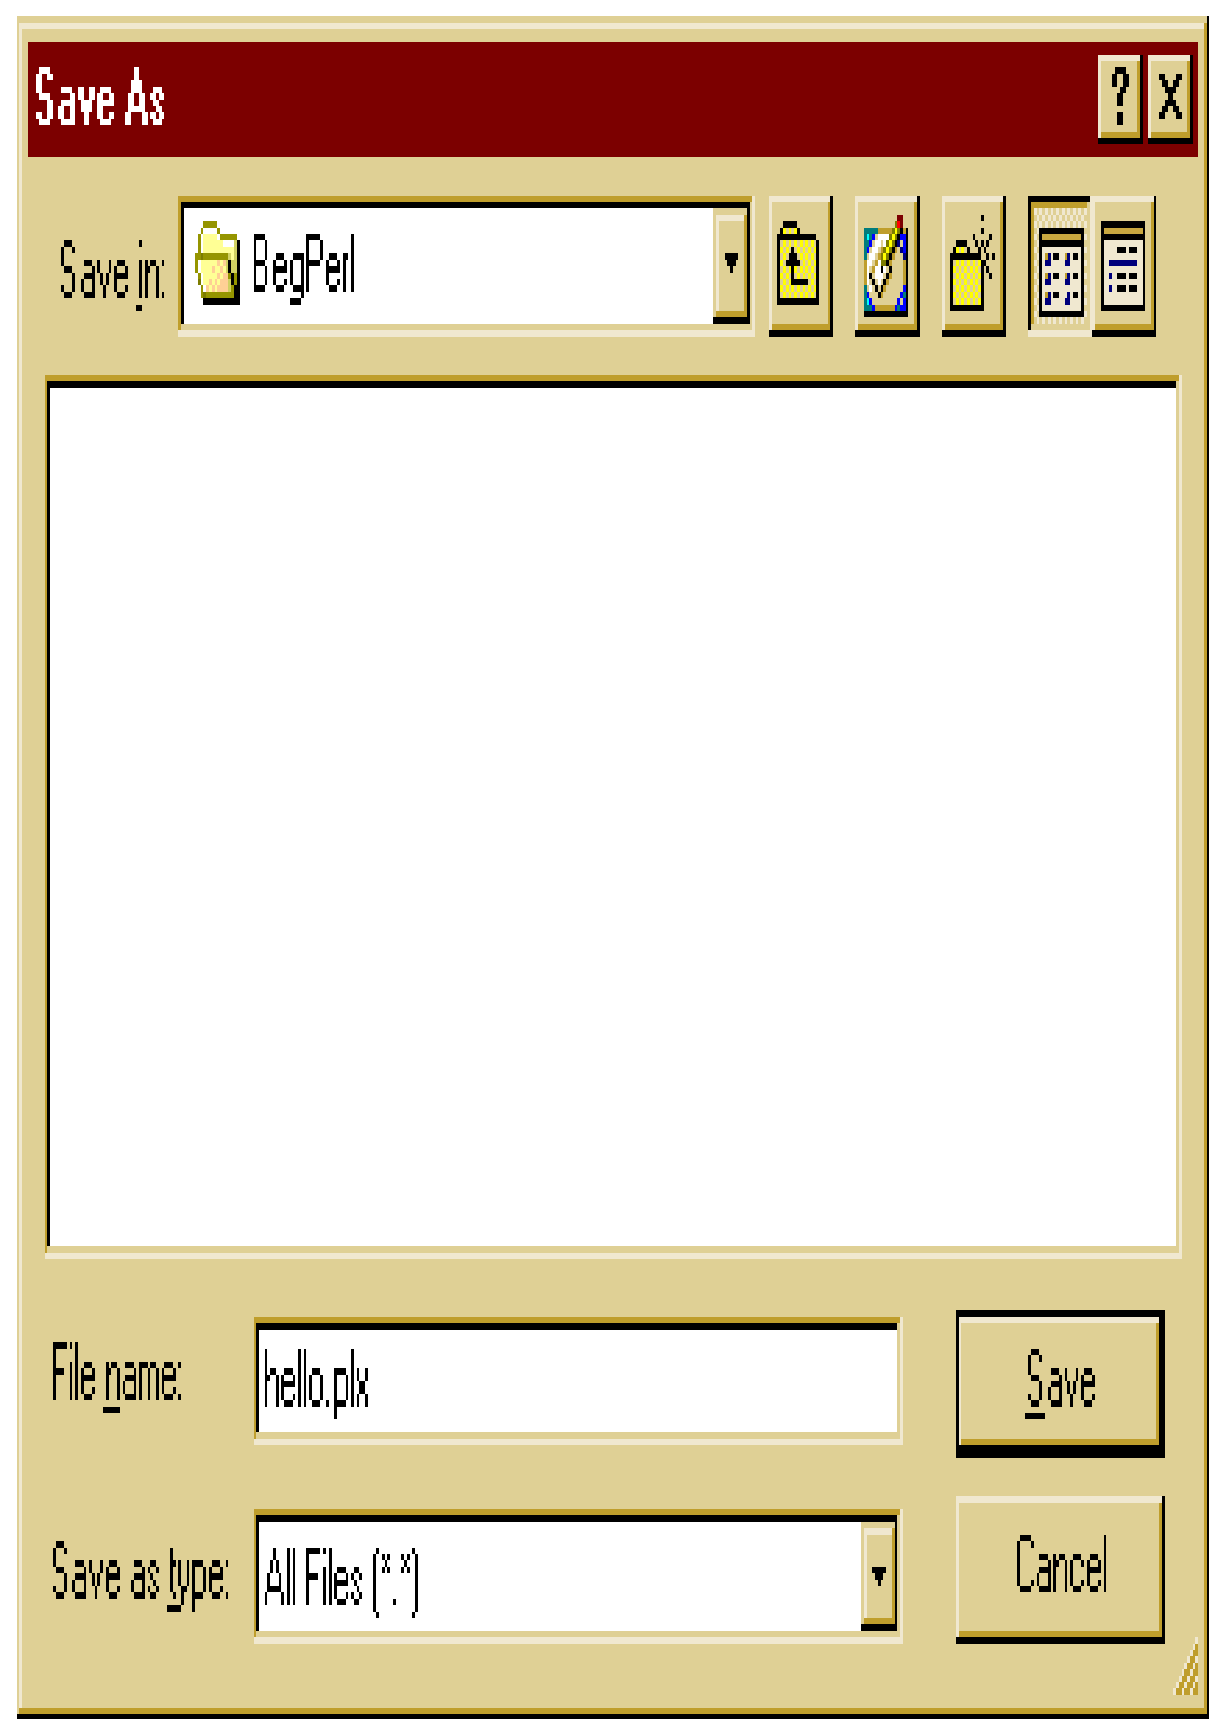
\includegraphics[bb=0mm 0mm 208mm 296mm, width=185.2mm, height=196.3mm, viewport=3mm 4mm 205mm 292mm]{image5.ps}

\noindent 

\noindent This work is licensed under the Creative Commons Attribution-NoDerivs-NonCommercial License. To view a copy of this

\noindent license, visit http://creativecommons.org/licenses/by-nd-nc/1.0 or send a letter to Creative Commons, 559 Nathan Abbott Way, Stanford, California 94305, USA.

\noindent 

\noindent The key terms of this license are:

\noindent 

\noindent Attribution: The licensor permits others to copy, distribute, display, and perform the work. In return, licensees must give the original author credit.

\noindent 

\noindent No  Derivative  Works: The licensor permits others to copy, distribute, display and perform only unaltered copies of the work -- not derivative works based on it.

\noindent 

\noindent Noncommercial: The licensor permits others to copy, distribute, display, and perform the work. In return, licensees may not use the work for commercial purposes -- unless they get the licensor's permission.


\end{document}

